\section{Progettazione dell'applicazione}
\subsection{Descrizione dell'architettura}
L'applicazione realizzata è stata scritta in linguaggio Java e si interfaccia con il database usando lo strumento di ORM Hibernate. Il database risiede in locale e come DBMS è stato scelto MySQL. Dal punto di vista architetturale l'applicazione implementa il pattern MVC: è quindi la parte di Controller ad occuparsi di interagire con il database.
\medskip

La schermata iniziale presenta 4 pulsanti che permettono di iniziare una nuova partita, continuare una partita in corso, visualizzare statistiche relative alle partite giocate e chiudere l'applicazione.

\begin{figure}[ht]
    \centering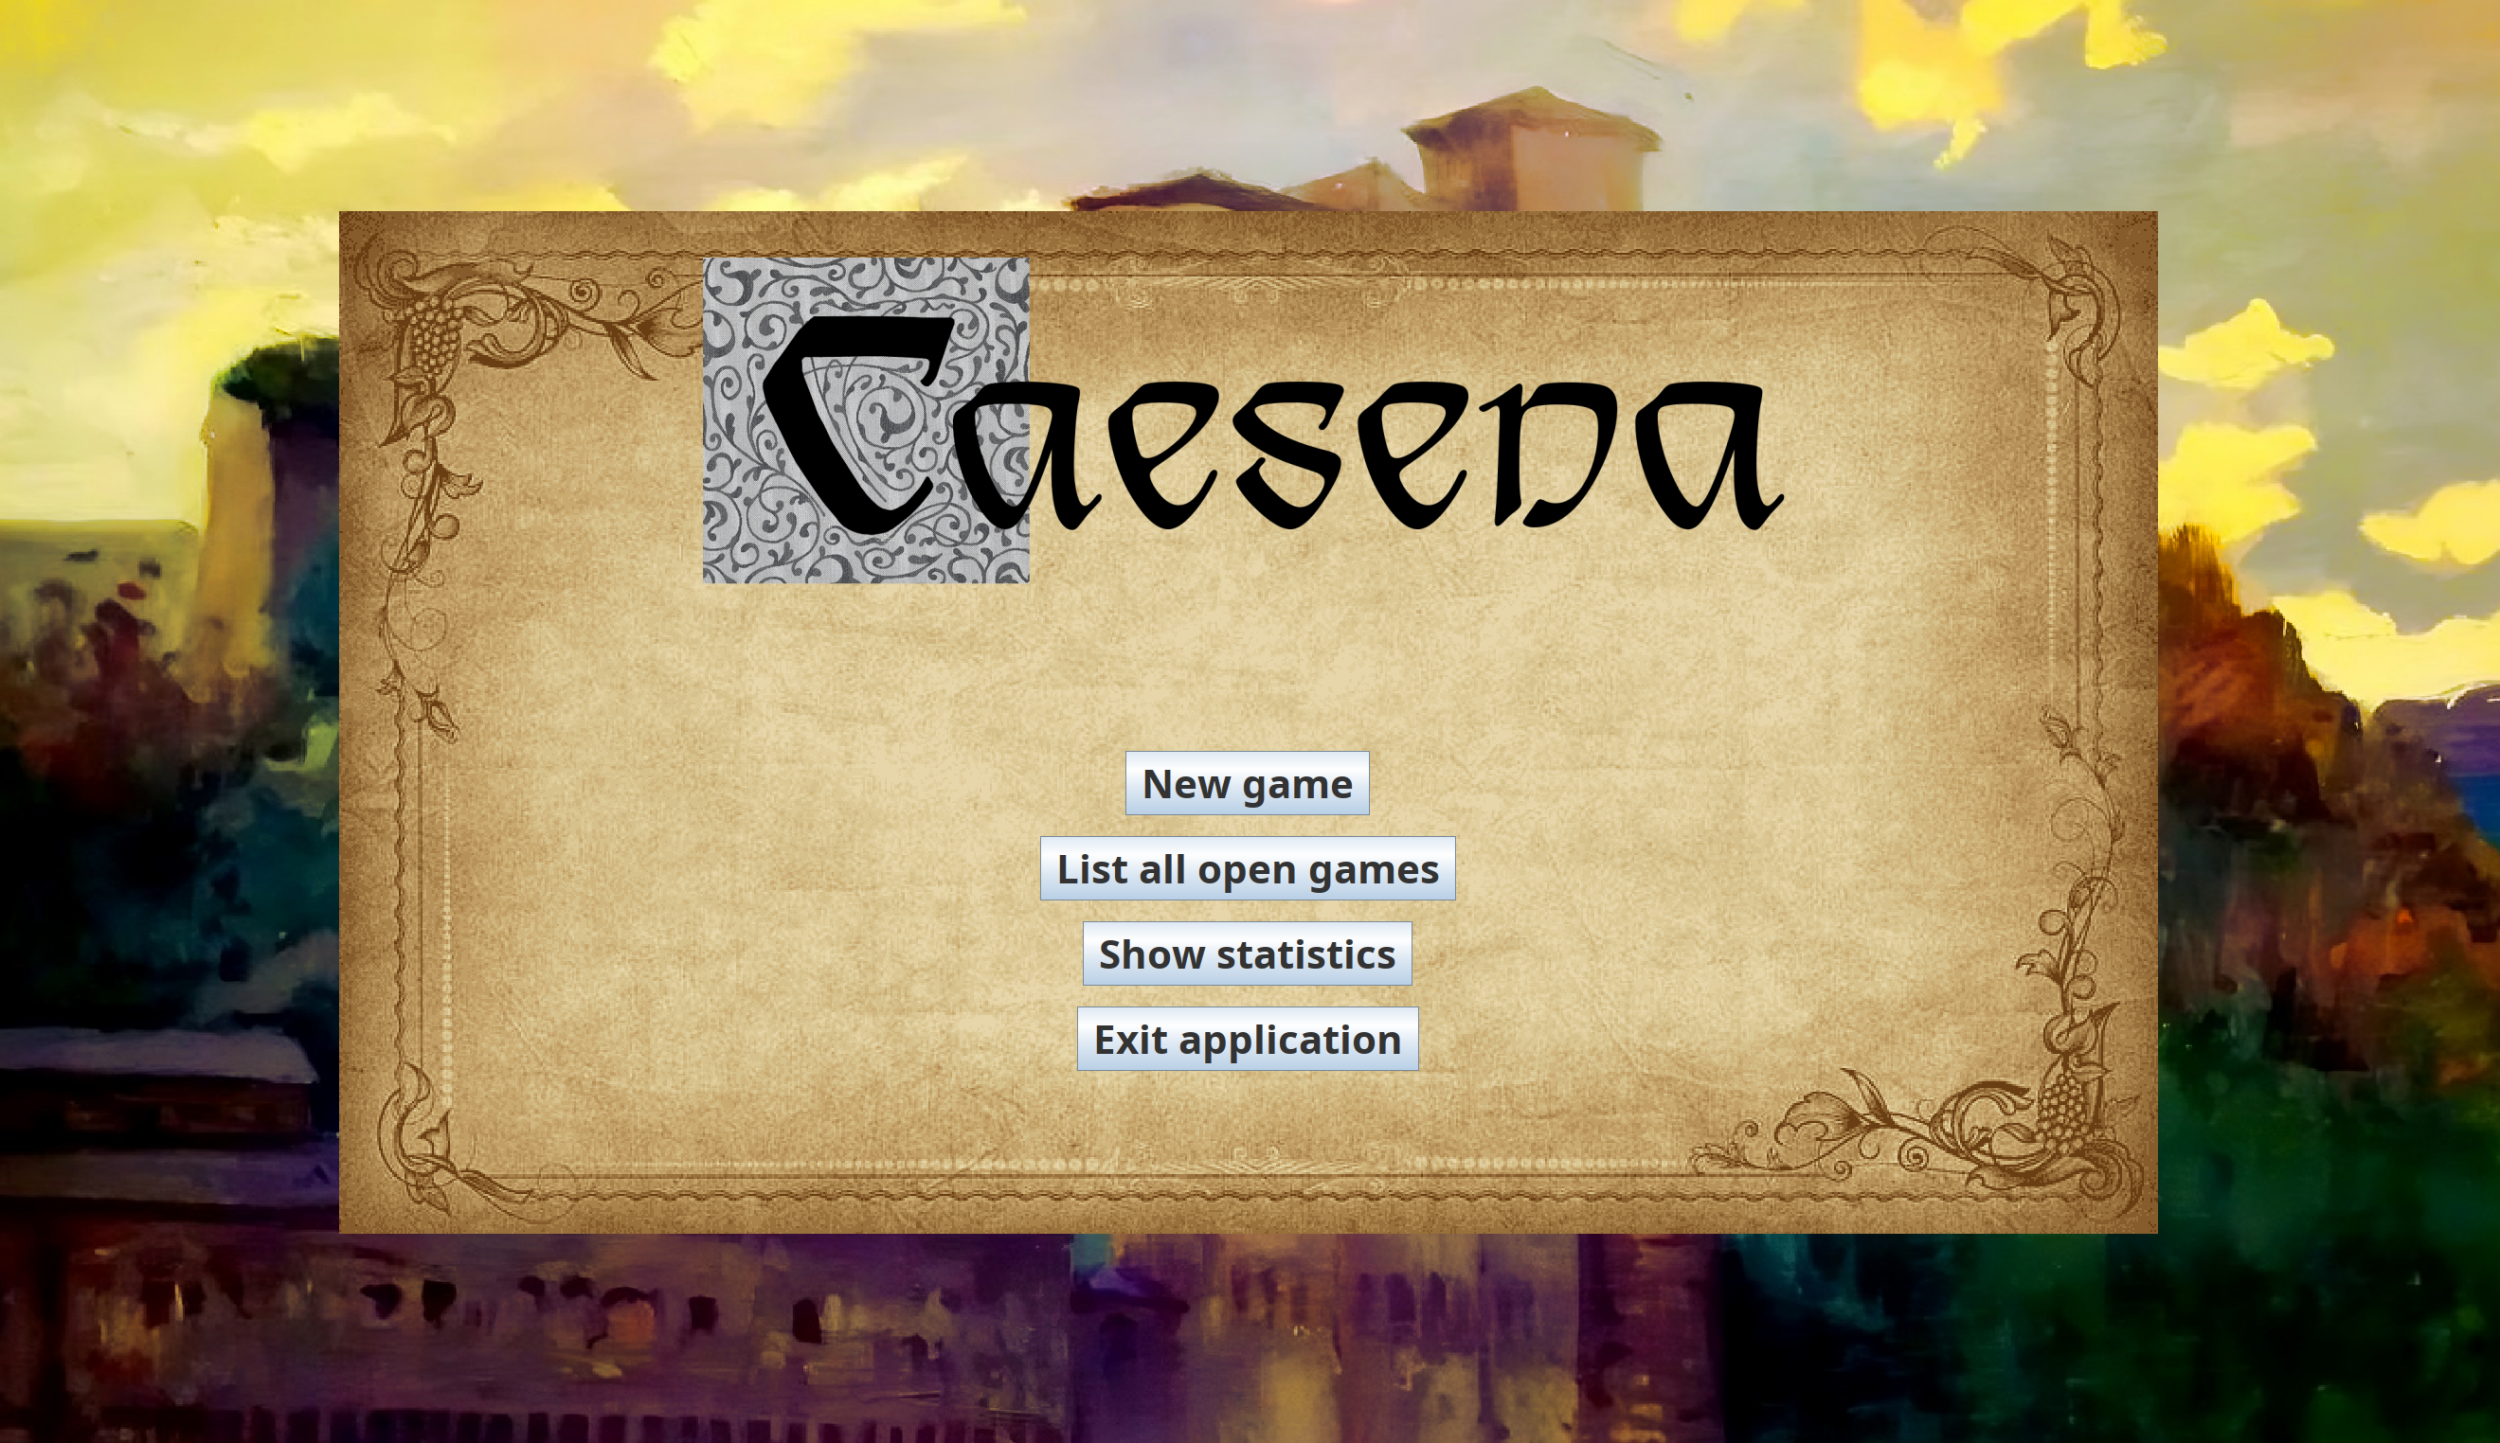
\includegraphics[scale=0.2]{images/startView.png}
\end{figure}

La schermata per l'inizio di una nuova partita presenta la scelta del server in cui giocare la partita, le espansioni da usare, il numero di giocatori, e per ciascuno, dei campi in cui inserirne il nome e il relativo colore. Dopo aver selezionato e impostato a piacimento le informazioni dei giocatori, si dovrà semplicemente cliccare sul pulsante "Inizia una nuova partita".

\begin{figure}[ht]
    \centering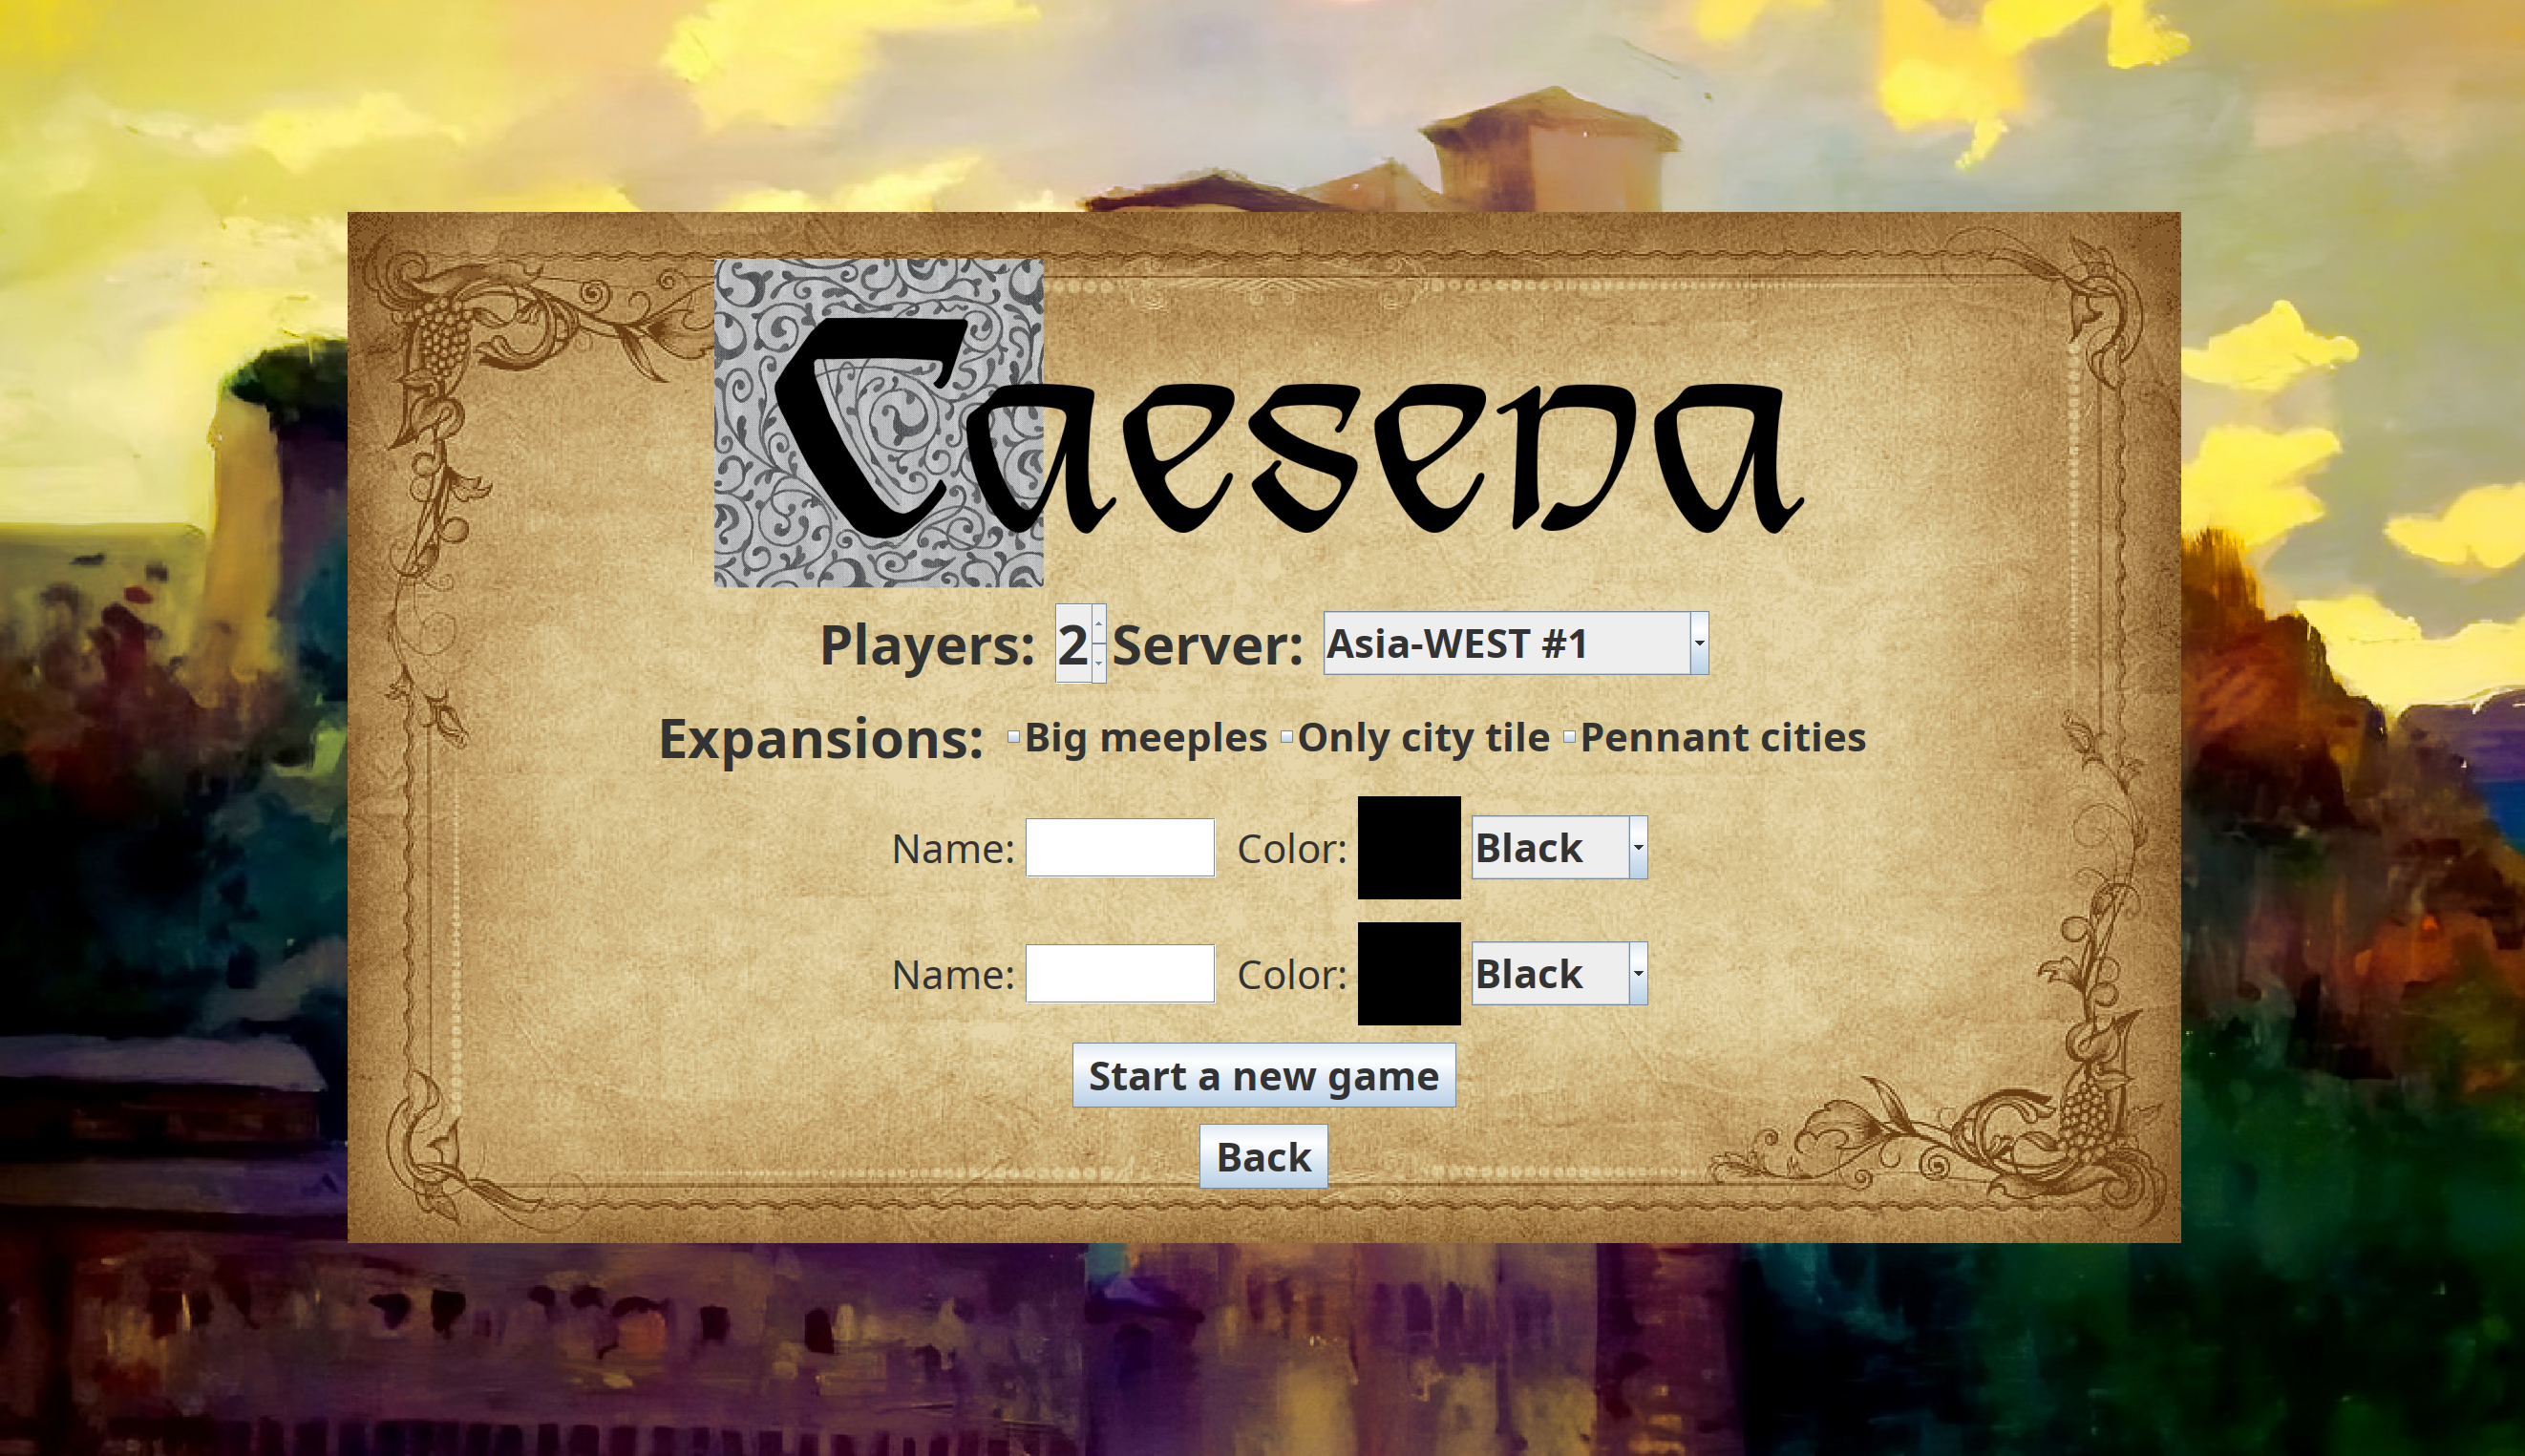
\includegraphics[scale=0.2]{images/newGamePage.png}
\end{figure}

La schermata per il proseguimento di una partita in corso presenta una casella combinata per scegliere di quale giocatore si vuole visualizzare l'elenco delle partite in corso. Apparirà quindi una tabella in cui in ogni riga saranno presenti le informazioni di una partita diversa ed un pulsante "Unisciti".

\begin{figure}[ht]
    \centering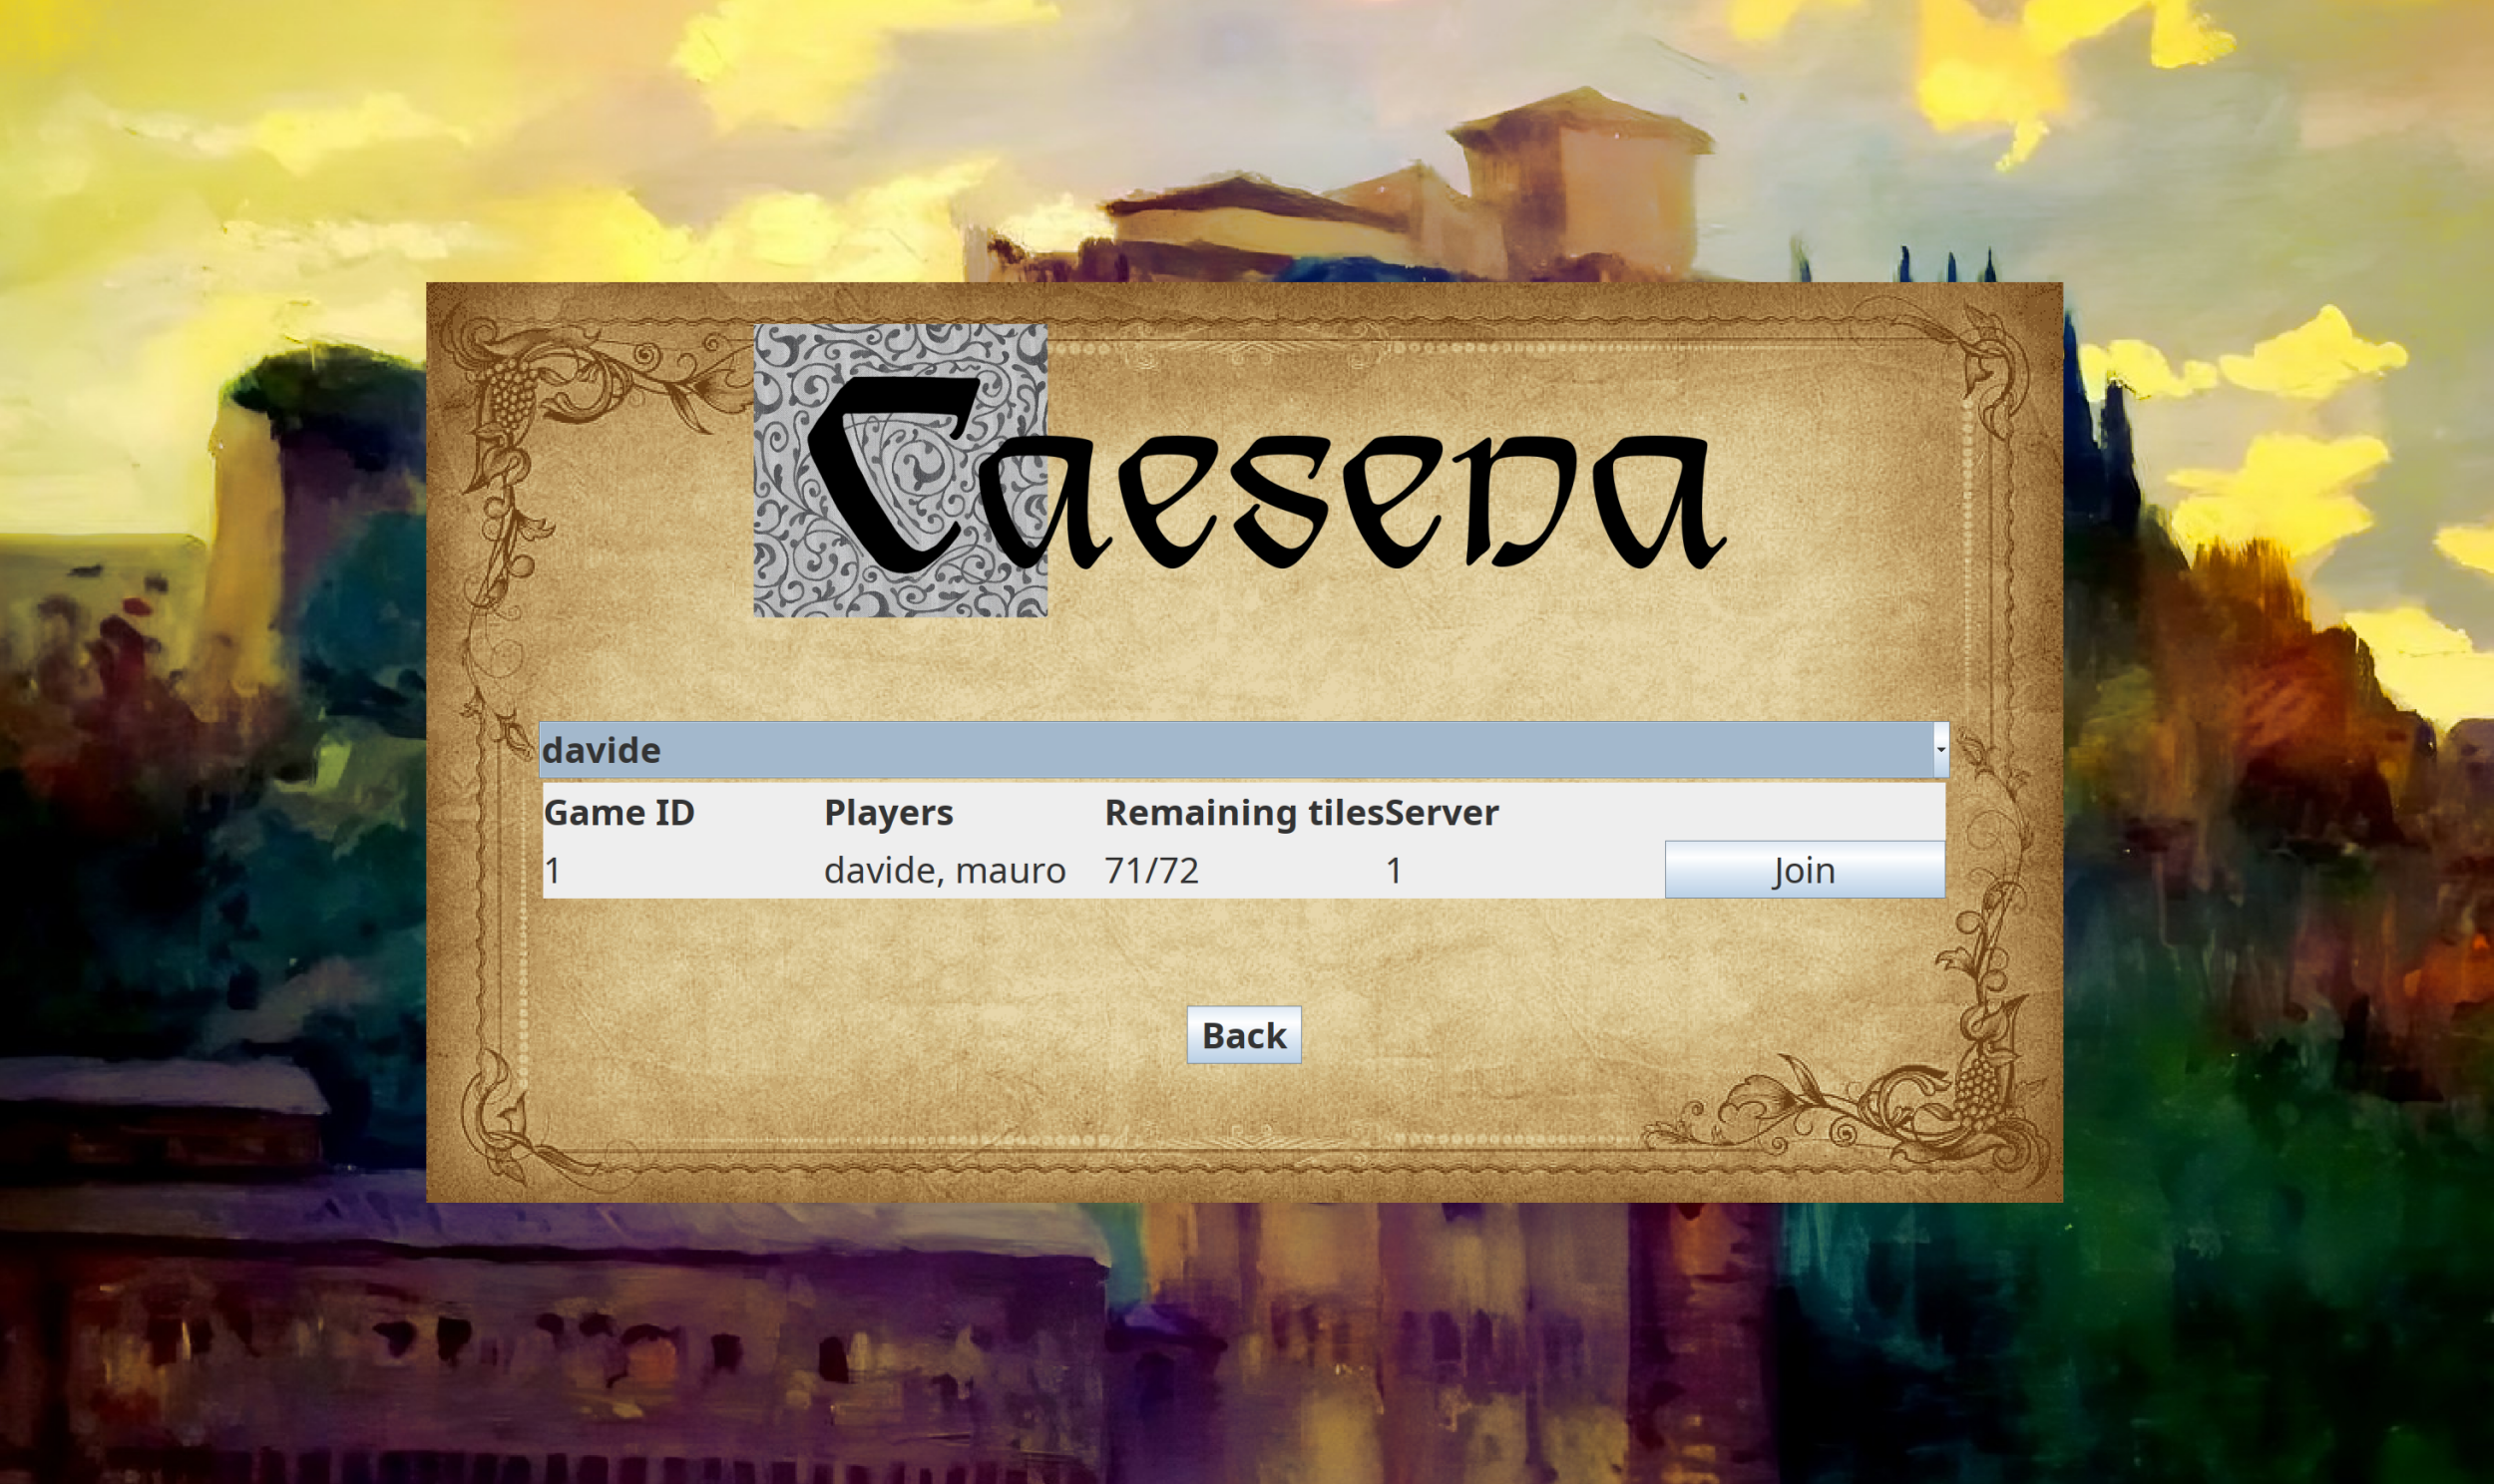
\includegraphics[scale=0.2]{images/gameListPage.png}
\end{figure}

La schermata per la visualizzazione di statistiche relative alle partite giocate presenta una tabella diversa per ognuna di esse. Degli esempi di statistiche sono l'espansione non base più giocata in ogni regione e con quanti altri giocatori diversi ogni giocatore ha giocato.

\begin{figure}[ht]
    \centering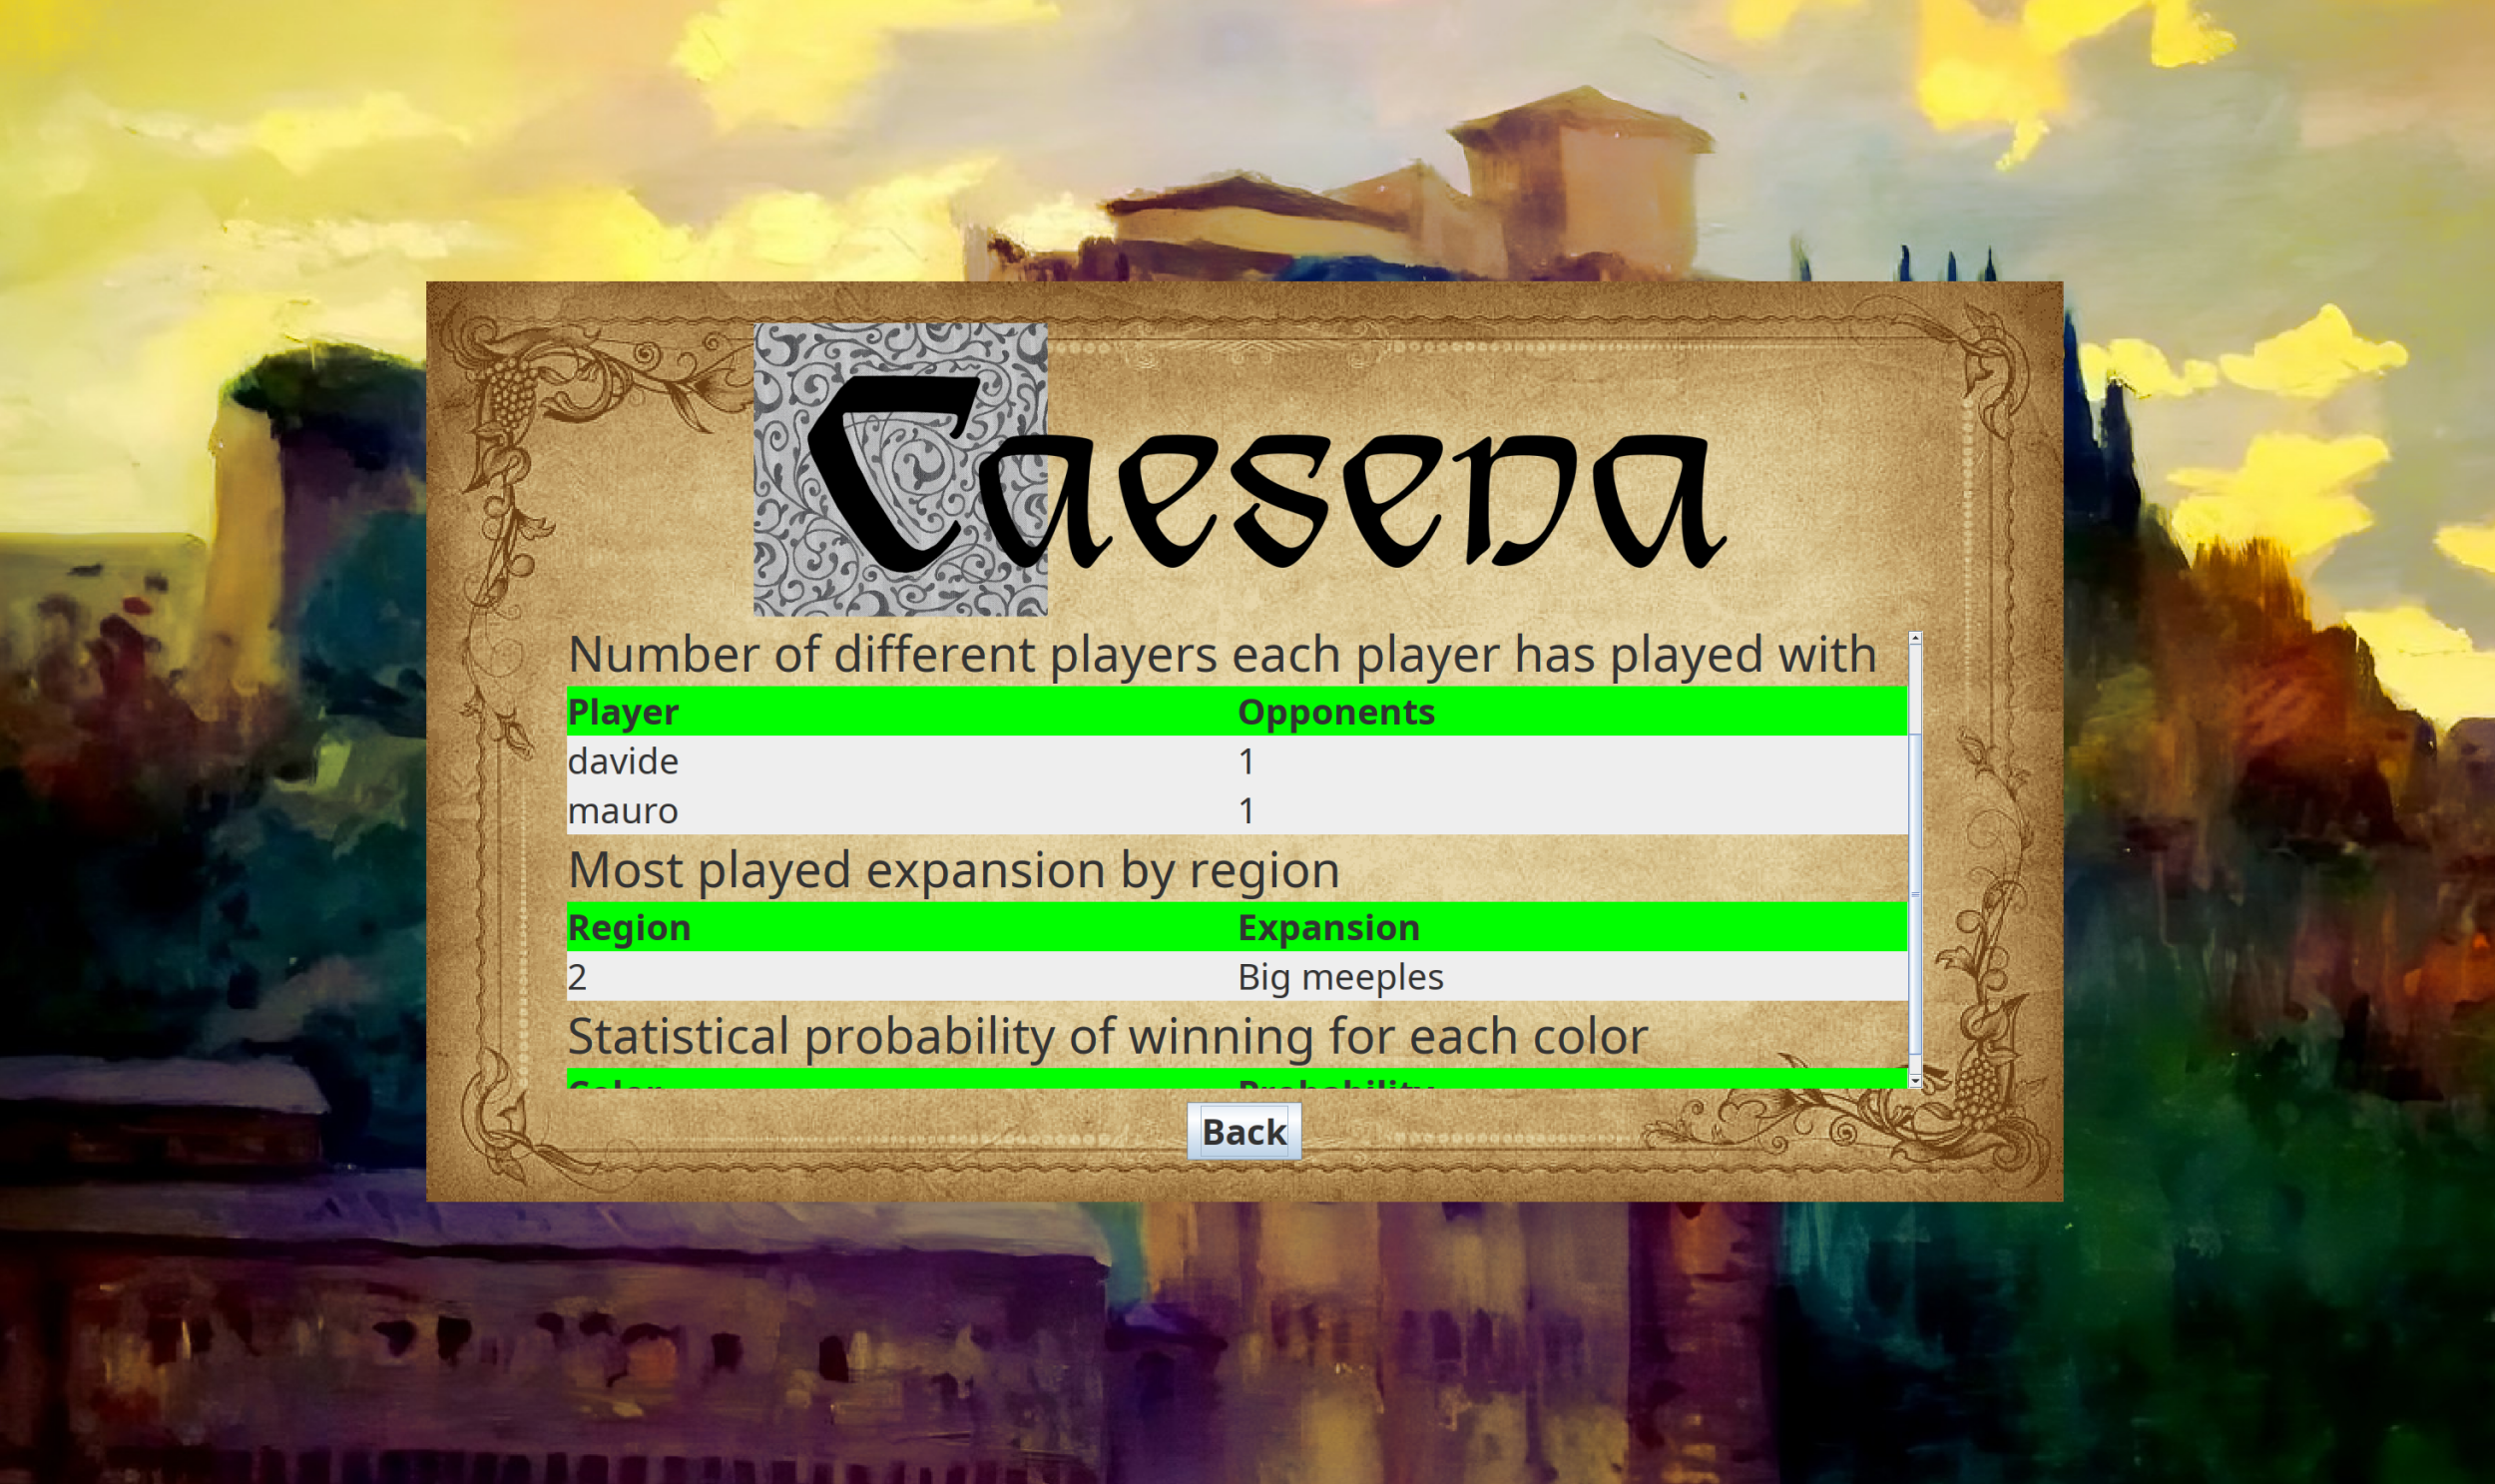
\includegraphics[scale=0.2]{images/statisticsPage.png}
\end{figure}

Una volta avviata la partita verrà mostrata la schermata di gioco il quale contenuto principale è il tabellone che mostra le tessere piazzate con i relativi seguaci sopra. In basso a sinistra dello schermo vengono mostrati colore e nome del giocatore corrente con i suoi seguaci, mentre alla destra si trovano la classifica dei giocatori e l'immagine della tessera corrente con il pulsante per ruotarla. A destra dello schermo si presentano invece i controlli del tabellone che ne gestiscono lo Zoom e ne permettono lo spostamento al suo interno. Premendo il pulsante "Piazza tessera" questa verrà piazzata solo in caso sia stata selezionata una posizione corretta nel tabellone. Premendo invece il pulsante "Scarta" verrà scartata la tessera solo se non piazzabile. Dopo aver piazzato la tessera apparirà la casella combinata che permette di scegliere il tipo di seguace da piazzare quando si preme il pulsante "Piazza seguace".

\begin{figure}[ht]
    \centering\includegraphics[scale=0.2]{images/gameView.png}
\end{figure}

Alla fine della partita, verrà mostrata la classifica finale nella quale ogni giocatore vedrà il proprio punteggio conclusivo e avrà la possibilità di tornare alla schermata iniziale o di uscire dal gioco.
\medskip

Il gioco supporta anche la lingua inglese nel caso il sistema operativo non utilizzi la lingua italiana, il testo dei pulsanti alla quale si riferisce questo capitolo si traduce nel seguente modo:
\begin{itemize}
    \item "Inizia una nuova partita" → "Start a new game"
    \item "Unisciti" → "Join"
    \item "Piazza tessera" → "Place tile"
    \item "Scarta" → "Discard"
    \item "Piazza seguace" → "Place meeple"
    \item "Finisci turno" → "End turn"
\end{itemize}
